The Simplex Method is a popular algorithm to solve linear programs first
published by Dantzig \cite{dantzig_maximization_1951}. Conceptually, it is quite
intuitive, especially from a geometrical point of view. I'll introduce the
method first in simple terms to provide a general idea before being a bit more
formal. Let us begin by discussing the example provided in the previous section.

We have the linear program:

%%% 
\begin{subequations}\label{eqs:lp}
  \begin{align}
    %%
    \min \:\: & 
    f(x_1, x_2) = 3 x_1 + 2 x_2
    & \label{eqs:lp_obj} \\
    %%
    \text{s.t.} \:\: &
    -2 x_1 + x_2 \leq 1 \\
    %%
    &
    x_1 + x_2 \leq 5 
    & \label{eqs:lp_sup} \\
    %%
    &
    x_1 \in [0, 4]
    &\label{eqs:lp_x1} \\
    %%
    &
    x_2 \geq 0
    &\label{eqs:lp_x2}
    %%
  \end{align}
\end{subequations}
%%% 
 
Which appears geometrically as:

\begin{figure}[H]
  \begin{center}
    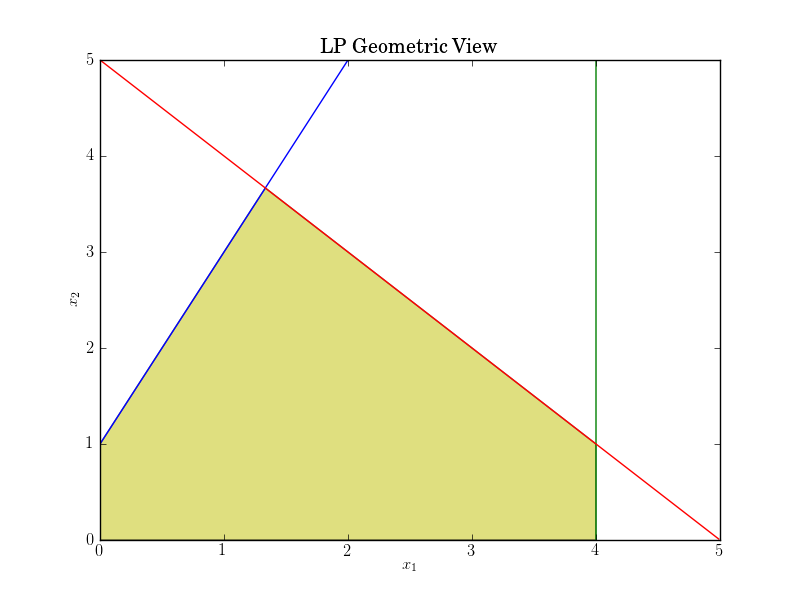
\includegraphics[width=\linewidth]{./chapters/litreview/plots/geometric.png}
  \caption{A Geometric View of the LP.}
  \label{fig:geometric}
  \end{center}
\end{figure}

Note that there are five vertices:

\begin{enumerate}
  \item $(0, 0)$
  \item $(0, 1)$
  \item $(\frac{4}{3}, \frac{11}{3})$
  \item $(4, 1)$
  \item $(4, 0)$
\end{enumerate}

The Simplex Method begins at a vertex, for example $(0, 0)$, and evaluates the
objective function.

\begin{equation}
    f(0, 0) = 3 * 0 + 2 * 0 = 0 
\end{equation}

Neighbor vertices are then evaluated, in order to determine which provides the
larger value (in the case of maximizing objectives).

\begin{equation}
    f(0, 1) = 3 * 0 + 2 * 1 = 2 
\end{equation}

\begin{equation}
    f(4, 0) = 3 * 4 + 2 * 0 = 12 
\end{equation}

The vertex $(4, 0)$ provides a larger objective function value, so the algorithm
moves to this vertex and determines the next largest neighbor. In this simple
example, there is only one choice, and it is trivially larger.

\begin{equation}
    f(4, 1) = 3 * 4 + 2 * 1 = 14 
\end{equation}

Accordingly the algorithm moves a second time, analyzing the neighboring
vertices again.

\begin{equation}
    f(\frac{4}{3}, \frac{11}{3}) = 3 * \frac{4}{3} + 2 * \frac{11}{3} = \frac{34}{3} 
\end{equation}

At this last move, a terminating condition has been achieved: a vertex has been
found for which all of its neighbors provide a lower value for the objective
function, i.e.,

\begin{equation}
    14 \geq 12 \:\:\: \text{and} \:\:\: 14 \geq \frac{34}{3}.
\end{equation}

Thus, the optimal value for $(x_1, x_2)$ has been determined to be $(4, 1)$. It
is immediately obvious that the simplex algorithm in this state is a hill
climbing (or hill descending) algorithm. The chief reason why this is possible
(i.e., why one is guaranteed to find a globally optimum solution) is that the
objective function and constraints are \textit{convex} functions of the decision
variables. Convexification is a requirement for optimum solutions to both linear
and integer programs, and the tightest possible set of constraints for a given
program describes its \textit{convex hull}.
